
% \chapter{Um apêndice}

    % Segundo a norma da ABNT (Associação Brasileira de Normas Técnicas), a definição e utilização de apêndices e anexos seguem critérios específicos para a organização de documentos acadêmicos e técnicos.
    
    % Apêndice: O apêndice é um texto ou documento elaborado pelo autor do trabalho com o objetivo de complementar sua argumentação, sem que seja essencial para a compreensão do conteúdo principal do documento. O uso de apêndices é indicado para incluir dados detalhados como questionários, modelos de formulários utilizados na pesquisa, descrições extensas de métodos ou técnicas, entre outros. Os apêndices são identificados por letras maiúsculas consecutivas, travessão e pelos respectivos títulos. A inclusão de apêndices visa a fornecer informações adicionais que possam ajudar na compreensão do estudo, mas cuja presença no texto principal poderia distrair ou desviar a atenção do leitor dos argumentos principais.

\chapter{Experiment 2}
    
    \section{Dataset}

    \begin{landscape}
    \scriptsize
        \begin{longtable}{|p{3cm}|p{22cm}|}
        \caption{Dataset used in the thesis experiments (Landscape).}\label{tab:dataset_landscape} \\
        \hline \textbf{Question} & \textbf{Ground Truth} \\ \hline
        \endfirsthead
        \multicolumn{2}{c}%
        {{\tablename\ \thetable{} -- Continued from previous page}} \\
        \hline \textbf{Question} & \textbf{Ground Truth} \\ \hline
        \endhead
        \hline \multicolumn{2}{|r|}{{Continued on next page}} \\ \hline
        \endfoot
        \hline \hline
        \endlastfoot
        % --- Data Starts Here ---
        Cite acidentes envolvendo colisão entre top drive e outros equipamentos. & 
        1. Colisão do Top Drive com Coluna de Produção na Mesa Auxiliar
        Durante a montagem de coluna de produção 6 5/8" na mesa auxiliar, o top drive colidiu com o último tubo acunhado na mesa rotativa, causando empenamento do tubo. A causa foi falha de planejamento e avaliação de risco, pois o top drive não foi retraído totalmente antes da descida. 
        \newline 2. Colisão entre o Top Drive e a Hydraracker
        Durante manobra de descida de coluna de Drill Pipe 5", o top drive colidiu com o braço principal da Hydra Racker que estava sendo estendido. A colisão provocou o desprendimento entre o braço principal e o braço inferior da Hydra Racker, com queda de uma peça de 2,7kg de altura de 27m. Causas incluíram operação em modo manual e configuração inadequada do sistema anticolisão.
        \newline 3. Colisão do Top Drive com Seção de Drill Pipe
        Durante manobra de retirada do BHA de 8 7/8", o top drive colidiu com a seção de Drill Pipe sustentada pelo PRS (Pipe Racking System). Com o impacto, a carenagem frontal do top drive foi cisalhada e caiu no piso do rigfloor de uma altura de 20m, pesando aproximadamente 85kg. 
        \newline 4. Interação do Top Drive Auxiliar com Equipamentos de Segurança
        Durante conexão de mangueira MPD, o cabo da trava quedas de um plataformista ficou preso no arranjo de içamento do top drive auxiliar, provocando a suspensão do trabalhador. O incidente ocorreu por falha na análise de risco e comunicação inadequada. \\ \hline        
        Quais as causas e falhas típicas de acidentes ou incidentes envolvendo guarda corpo?  Cite alertas que retratem isso. & 
        Os acidentes ou incidentes envolvendo guarda-corpo geralmente ocorrem devido a falhas de projeto, gestão de processos, especificação inadequada do serviço, e falta de procedimentos específicos. Aqui estão algumas causas e falhas típicas.
        \newline 1. Falha de Equipamentos e Projeto de Engenharia Deficiente: O projeto do guarda-corpo pode não ser adequado para a operação, levando a deslocamentos inesperados e acidentes. (Fonte: Definitivo - Lesão no dorso do pé direito devido ao choque com guarda corpo\_ POCOS SM \_Abrange+2023-000154)         
        \newline 2. Falha na Gestão de Processos e Pessoas: Inclui falhas no processo de qualificação da empresa contratada, violação de procedimentos por supervisores, e falta de documentos específicos para avaliação de operações. (Fonte: Definitivo - Lesão no dorso do pé direito devido ao choque com guarda corpo\_ POCOS SM \_Abrange+2023-000154)         
        \newline 3. Falha de Identificação de Risco Adicional de Queda: Não identificar riscos adicionais, como vãos entre a gaiola da escada e o guarda-corpo, pode resultar em quedas fatais. (Fonte: Acidente fatal-Queda de altura - REVAP-MA-PM\_ Abrange 2023-000279)         
        \newline 4. Movimento Irregular da Carga e Falha no Freio do Guindaste: Durante movimentações de carga, falhas no equipamento podem causar impactos que danificam o guarda-corpo e resultam em quedas de objetos. (Fonte: Alerta Definitivo - Vermelho - Descida descontrolada de carga - Divulgação equipe movimentação carga) \\ \hline
Quais foram as principais falhas identificadas em acidentes com pés, de acordo com os Alertas de SMS? & As principais falhas identificadas em acidentes envolvendo pés incluem:        
        \newline 1. Planejamento inadequado e falta de análise de risco: Muitos acidentes ocorreram devido à falta de planejamento adequado e análise de risco antes de realizar atividades, como movimentação de cargas e içamento de peças. Isso foi observado em acidentes como o de fratura em três metatarsos do pé esquerdo durante a fabricação de um corrimão na oficina de solda ("Preliminar AMARELO - Acidente com Lesão - Fratura - Geral - POCOS SM 055 2022").        
        \newline 2. Uso inadequado de Equipamentos de Proteção Individual (EPI): Em alguns casos, o uso inadequado ou a falta de EPI apropriado, como botas de segurança com proteção para metatarso, contribuiu para a ocorrência de acidentes. Isso foi destacado em acidentes como o corte contuso no pé esquerdo durante a manutenção de um gerador ("Definitivo AMARELO - Corte contuso no pé\_ Geral\_ POCOS SM 019\_rev01").        
        \newline 3. Falta de percepção de riscos e consciência situacional: A falta de percepção de riscos e a escolha de caminhos mais curtos sem avaliar o ambiente contribuíram para acidentes, como a torção no tornozelo ao pisar em uma madeira de apoio de carga ("Definitivo -Torção no tornozelo ao pisar sobre uma peça de madeira - POCOS SM 025 2023").        
        \newline 4. Falhas na supervisão e no cumprimento de diretrizes: A supervisão inadequada e o não cumprimento de diretrizes e procedimentos de segurança foram fatores em acidentes, como o de fratura no tornozelo ao tropeçar em um umbilical no convés ("Definitivo VERMELHO - Fratura no tornozelo\_Geral\_ POCOS SM 016 2021").
        \newline 5. EPI Inadequado: Uso de botas sem características anti-torção e solado adequado para ambientes offshore, como mencionado no acidente de torção de tornozelo ao descer escada (POCOS SM 009 2021). \\ \hline  
Como a presença de sílica na composição da pasta de cimento afeta sua estabilidade térmica em altas temperaturas, de acordo com as lições aprendidas? & A sílica é adicionada ao cimento na proporção de 35\% por peso de cimento com o objetivo de mitigar a retrogressão (perda da resistência compressiva) do cimento no poço quando submetido a temperaturas superiores a 230°F (110°C). Esta prática é comum em poços profundos ou com gradiente geotérmico elevado que, em suas fases finais, ultrapassam a temperatura limite. A presença de sílica na pasta de cimento também pode ser necessária em situações onde a temperatura nos anulares dos revestimentos durante a produção do poço seja bastante elevada, mesmo em menores profundidades.
        \newline        A ausência de sílica no cimento sujeito a temperaturas superiores a 230°F pode resultar numa perda de resistência compressiva no cimento, levando a problemas de isolamento.
        \newline        Entretanto, é importante observar que a má preparação da pasta de cimento pode resultar em propriedades da pasta inhomogêneas durante a fabricação e bombeamento. Isso pode levar a gelificação prematura e possível prisão da coluna. Em caso de anormalidades na preparação da pasta, recomenda-se a realização da cimentação em bateladas.
        
        Referências:
        \newline        Alerta Técnico AT5533: Utilização de cimento com sílica na cimentação de revestimentos de superfície. Autor: Jan Fernandes Aslan. Data: 16/11/2020.
        \newline        Alerta Técnico AT10479: Substituição indevida de cimento com sílica por cimento puro em cimentação de revestimento de superfície em poço com temperatura elevada. Autor: Rafael Peralta Muniz Moreira. Data: 14/02/2021.
        \\ \hline

De acordo com as lições aprendidas, como a inclinação do poço afeta a eficácia da cimentação durante o tamponamento through tubing? & Durante o tamponamento through tubing em poços de alta inclinação (maior que 45 graus), a eficácia da cimentação pode ser afetada por fatores advindos da inclinação do poço. Segundo um Alerta Técnico (AT9613), essa situação aumenta a complexidade das operações de tamponamento devido ao fato de a coluna de produção/injeção estar descentralizada dentro do revestimento de produção. 
        \newline        Além disso, outras dificuldades surgem, como:
        \newline        - Dificuldade no assentamento de cement retainer inflável
        - Dificuldade na descida de ferramentas de perfilagem e plugs para isolamento preliminar abaixo do trecho do poço a ser tamponado
        \newline        Estes fatores podem resultar em poços com qualidade média ou falha na cimentação. Recomenda-se por agora, até que estudos mais aprofundados sejam realizados, uma análise criteriosa de cada cenário e a escolha de alternativas mais robustas para o abandono de poços de alta inclinação e a seleção de escopo de projeto executivo de abandono, detalhamento operacional e estimativa dos riscos e tempos da intervenção.
        \newline        Por outro lado, existem algumas alternativas como o Bombeio Direto de Cimento (BDC) para abandono permanente through tubing (TT). Isso permite o bombeio de pasta de cimento diretamente pelo riser dual bore, passando pela COP/COI até ser posicionada em anular “A” (COP x revestimento). No entanto, essa técnica também tem suas restrições e premissas, como necessidade de emprego de Riser Dual Bore e menor tolerância ao erro no deslocamento de pasta.
        \newline        Em resumo, a inclinação do poço pode afetar a eficácia da cimentação durante o tamponamento através do tubo, tornando a operação mais complexa e aumentando o risco de falhas na cimentação. Diferentes abordagens e tecnologias estão sendo estudadas para otimizar essas operações e minimizar os riscos. \\ \hline

De acordo com as lições aprendidas, quais são os riscos associados à substituição de cimento com sílica por cimento puro em cimentações de revestimento de superfície em poços com temperatura elevada? & Estes são os principais riscos associados à substituição indevida de cimento com sílica por cimento puro em poços de alta temperatura:
        \newline        1. O cimento puro, quando submetido a altas temperaturas (acima de 110°C), sofre uma regressão de sua resistência compressiva ao longo do tempo, podendo comprometer sua função em poços de petróleo como elemento de barreira.
        \newline        2. Falhas na cimentação do revestimento de superfície podem levar a custos e impactos adicionais, como o vazamento de fluidos de perfuração para o fundo do mar e o aumento das cargas hidrostáticas sobre o revestimento de superfície e os revestimentos subsequentes instalados.
        \newline        3. Em alguns casos, a bainha de cimento pode ser exposta a temperaturas acima de 110°C em algum momento do ciclo de vida do poço. Nesses casos, o uso de cimento com sílica deve ser mantido para garantir a estabilidade térmica da pasta de cimento.
        \newline        4. A substituição indevida pode levar a outros riscos como escape de fluidos de perfuração do anular C para o fundo do mar, alterações no dimensionamento do revestimento, alterações no desenho de projeto de início de poço, entre outros.
        \newline        Deve-se ressaltar que a intenção de reduzir o tempo de aguardo de cura do cimento não justifica a substituição do cimento com sílica por cimento puro, pois existem outros métodos para alcançar uma cura mais rápida, como o aumento da densidade da pasta ou o uso de aditivos.
        \newline        Esse fenômeno é conhecido na indústria do petróleo desde 1954 e foi mitigado pela introdução de sílica cristalina na composição da pasta de cimento para garantir a estabilidade térmica. \\ \hline

Quais estratégias podem ser adotadas para melhorar a qualidade da cimentação em poços de alta inclinação durante o tamponamento through tubing, de acordo com as lições aprendidas? & Com base nos itens de conhecimento obtidos, algumas estratégias para melhorar a qualidade da cimentação em poços de alta inclinação durante o tamponamento through tubing incluem:
        \newline        1. Aumento das vazões no deslocamento quando a cimentação é executada com flexitubo. Este procedimento auxilia na melhor distribuição do cimento no espaço anular e contribui para uma melhor qualidade de cimentação.
        \newline        2. Utilização de dispositivos para vibração da coluna durante a cimentação. A vibração pode ajudar a melhorar a aderência do cimento no espaço anular tornando a cimentação mais eficaz.
        \newline        3. Utilização de volumes de excesso de pasta de cimento compatíveis com uma operação que busque robustez máxima. Este procedimento garante que haja cimento suficiente para preencher o espaço anular ao longo de todo o comprimento da coluna.
        \newline        4. Análise criteriosa de cada cenário e seleção de uma alternativa mais robusta para o abandono (preferencialmente com a retirada da coluna). Isso é particularmente importante para poços de alta inclinação e outros cenários que adicionem complexidade ao tamponamento.
        \newline        5. Previsão no cronograma da intervenção da perfilagem de avaliação da cimentação como método de verificação. Isso permite a identificação de possíveis falhas ou áreas de cimentação insatisfatória para um possível retoque da cimentação.
        \newline        6. Uso do Bombeio Direto de Cimento (BDC) para abandono permanente through tubing, uma técnica que pode otimizar o tempo e reduzir os riscos operacionais, embora com restrições específicas.
        \newline        Por último, é importante lembrar que toda situação é única e deve ser avaliada individualmente de acordo com as suas características específicas. \\ \hline

Quais são as alternativas para acelerar o tempo de cura da pasta de cimento sem comprometer sua integridade em condições de temperatura elevada, de acordo com as lições aprendidas? & As melhores práticas incluem o aumento da densidade da pasta, o uso de aditivos e a consideração da rampa de cura, mas é importante manter a utilização de cimento com sílica para garantir a integridade da cimentação em condições de temperatura elevada. \\ \hline

Quais são os principais desafios e riscos associados ao tamponamento through tubing em poços de alta inclinação, de acordo com as lições aprendidas? & Existem vários desafios e riscos associados ao tamponamento through tubing em poços de alta inclinação, conforme revelado no Alerta Técnico "Risco de falha de cimentação em tamponamento through tubing em poços de alta inclinação (45 graus)". Os principais problemas incluem:
        \newline        - Maior complexidade nas operações de tamponamento devido à descentralização da coluna de produção/injeção dentro do revestimento de produção em poços com alta inclinação.
        - Dificuldade no assentamento de cement retainer inflável em poços inclinados.
        - Dificuldade na descida de ferramentas de perfilagem e plugs para isolamento preliminar abaixo do trecho do poço a ser tamponado.
        \newline        Além disso, foi observado que em poços de alta inclinação (> 45 graus), a qualidade da cimentação é, muitas vezes, apenas média, cumprindo apenas os requisitos mínimos e, em alguns casos, levando a falhas na cimentação.
        \newline        No atual cenário, para melhorar os resultados, é sugerido o uso de vazões no deslocamento superiores quando a cimentação é realizada com flexitubo, a realização do uso de dispositivos para vibração da coluna durante a cimentação e o uso de volumes excedentes de pasta compatíveis com uma operação da maior robustez possível.
        \newline        Destaca-se também a importância do controle de circulação e perda de fluido durante a perfuração da fase do reservatório. Em situações de perda de circulação severa, a perfuração com água do mar e tampões viscosos pode ser uma alternativa segura para evitar custos e riscos adicionais.
        \newline        É relevante mencionar também o uso de métodos sustentáveis e eficientes de combate à perda de fluido pós-teste de formação, em que um tampão especial de filtrado relaxado pode ser uma solução viável, trazendo economia e eficiência operacional.
        \newline        No entanto, até que um estudo mais aprofundado sobre as causas desses problemas seja realizado e medidas de melhoria sejam implementadas, recomenda-se a seleção cuidadosa do plano de abandono e a análise prévia de cada cenário para poços de alta inclinação. \\ \hline
Cite problemas operacionais ocorridos na sonda NS-48 em 2024, de acordo com o SITOP? Liste todas as ocorrências que encontrar. & 1. Falha no Sistema de Rotação do Top Drive: Houve uma investigação contínua sobre uma falha no sistema de rotação do top drive, que impossibilitou a conexão à coluna. Durante o período de espera, o ponto de acunhamento da cunha foi alterado duas vezes. Fonte: <a href="https://wellsom.petrobras.com.br/sitopi/sonda/NS-48/2024-07-19/M" target="blank">Documento da sonda NS-48 - 2024-07-19 11:50</a>
        \newline        2. Condições Ambientais Adversas: Em várias ocasiões, as operações foram interrompidas devido a condições ambientais adversas, como ventos fortes, que impediram a montagem de equipamentos de arame e a retirada de plugues. Fonte: <a href="https://wellsom.petrobras.com.br/sitopi/sonda/NS-48/2024-05-09/M" target="blank">Documento da sonda NS-48 - 2024-05-09 07:30</a>
        \newline        3. Atrasos na Instalação de Equipamentos: Houve atrasos na instalação de equipamentos, como a ANM CCB-462, devido à espera por embarcações de apoio, o que impactou o cronograma das operações. Fonte: <a href="https://wellsom.petrobras.com.br/sitopi/sonda/NS-48/2024-05-21/M" target="blank">Documento da sonda NS-48 - 2024-05-21 05:24</a>
        \newline        4. Problemas com o WSSV Blue Marlim: A sonda enfrentou problemas operacionais devido à indisponibilidade do WSSV Blue Marlim para operar conectado, causada por condições de mar adversas e problemas no gerador do barco. Fonte: <a href="https://wellsom.petrobras.com.br/sitopi/sonda/NS-48/2024-04-13/T" target="blank">Documento da sonda NS-48 - 2024-04-13 13:29</a>
        \newline        5. Falha no sistema de rotação do top drive: Houve uma investigação sobre a falha no sistema de rotação do top drive, que impossibilitou a conexão à coluna. Durante o período de aguardo, o ponto de acunhamento da cunha foi alterado duas vezes. Fonte: <a href="https://wellsom.petrobras.com.br/sitopi/sonda/NS-48/2024-07-19/M" target="blank">NS-48 - 2024-07-19</a>
        \newline        6. Aguardando troca de turma: Houve um período de espera para troca de turma do WSSV Blue Marlim, durante o qual foram realizadas operações de mini-TI e recalcamento de fluidos. Fonte: <a href="https://wellsom.petrobras.com.br/sitopi/sonda/NS-48/2024-04-12/M" target="blank">NS-48 - 2024-04-12</a> \\ \hline

Em quais poços foi utilizado Well Stroker para abertura e fechamento de VIF, de acordo com o SITOP? Liste todas as ocorrências que encontrar. & Foram encontrados 6 poços com ocorrência de uso de Well Stroker para abertura e fechamento de VIF
        1. 8-BUZ-55-RJS
        2. 7-BAZ-3-ESS 
        3. 8-RO-146HP-RJS
        4. 7-CRT-52-RJS
        5. 8-BUZ-58D-RJS
        6. 7-JUB-61D-ESS
        7. 8-ATP-7D-RJS
        8. 3-RJS-688A \\ \hline

Em quais poços haverá cimentação de revestimento entre as próximas operações, de acordo com o SITOP do dia 13/05/2025? Informe somente a lista de nomes dos poços. Liste todos os poços que encontrar, não tente resumir. & Nos próximos dias, haverá operações de cimentação de revestimento nos seguintes poços:
        \newline        1. Poço 7-BUZ-95-RJS
        \newline        2. Poço 7-JUB-81H-ESS
        \newline        3. Poço 7-BUZ-94D-RJS
        \newline        4. Poço 8-MRO-36-RJS
        \newline        5. Poço 8-BUZ-101-RJS
        \newline        6. Poço 9-AB-138D-RJS
        \newline        7. Poço Buena Suerte-1
        \newline        8. Poço 7-BUZ-94D-RJS \\ \hline

Em qual poço está a sonda NS-39, de acordo com o SITOP? Considere que a data de hoje é 05/01/2025.  & A sonda NS-39 está operando no poço 7-MRO-37-RJS. \\ \hline

Quais as últimas operações efetuadas no poço 7-MRL-244H-RJS, de acordo com o SITOP do dia 05/01/2025? & Operação Principal:
        MP: Circulado FPBNA 9,4 ppg via coluna a 8 bpm / 270 psi.
        MP: Bombeado 50 bbl de colchão espaçador 11,0 ppg via bomba da sonda 6 bpm / 230 psi e deslocado com 10 bbl de FPBNA 9,4 ppg a 6 bpm / 230 psi pela bomba da sonda.
        MP: Bombeado 96 bbl de pasta de cimento 15,8 ppg a 4 bpm e deslocado com 6,9 bbl de colchão espaçador 11 ppg e com 59 bbl de FPBNA 9,4 ppg.
        MP: Retirada coluna até 939 m (mais de 200 m acima do TOC), circulado para limpeza da coluna com FPBNA 9,4 ppg e fechado BOP anular.
        MP: Bombeado via UC 68 bbl de FPBNA 9,4 ppg pela coluna e efetuando squeeze do cimento no overlap liner 10,75" x revestimento 13,626" a 1 bpm/ 260 psi, 2 bpm/ 330 psi, 3 bpm/ 340 psi e a 4 bpm/ 410 psi.  
        MP: Iniciado aguardo de pega de 11 h do cimento às 21:30 h.
        \newline        Operação Paralela:
        MA: Continuada montagem e estaleiramento do BHA 8 1/2". 
        MA: Iniciada montagem do Djar e de ferramenta de condicionamento do topo do liner.  \\ \hline

Quais foram as operações executadas na NS-42 em 22/06/2024, de acordo com o SITOP?  & 
        Descido conjunto FDR/TRT com coluna de DPR 6 5/8" até 936 m.
        Efetuado dummy run com coluna de DPR e ajustado balanceio.
        Conectada coflex na SFT.
        Efetuada plumbagem da SFT.
        Verticalizado arranjo de superfície com SFF, EBE, links articulados e conectado DPR 6 5/8" da SFT na coluna.
        Em paralelo, limpado TMF da ANM pelo ROV.
        Montado BOP de arame sobre a SFT.
        \newline        Finalizada montagem das linhas de superfície e manifold auxiliar.
        Efetuado teste de estanqueidade das linhas de superfície com 300 psi / 4500 psi por 5 min / 10 min.
        Efetuado teste de estanqueidade do DPR até as valvulas VG5 e XO da FDR com 3500 psi por 10 min. Hold Point aprovado pelo CSD-EQSB
        Efetuado flush do DPR e HCR para limpeza.
        Posicionado FCBA inibido com MEG 10% no interior do DPR e HCR.
        \newline        \\ \hline

Qual  o SITOP de hoje da NS-45? Considere que a data de hoje é 05/01/2025. & A situação operacional da sonda NS-45 em 05/01/2025 é a seguinte:
        \newline         Operação Principal
        - **Manutenção do BOP**: As manutenções do BOP estão 63% concluídas. As atividades incluem a limpeza dos receptáculos, stabs, troca das vedações da interface LMRP/Stack, troca dos packers seals do POD azul, manutenção das reguladoras do POD azul e amarelo, e lubrificação do riser connector.
        - **Situação Atual**: A operação está aguardando a substituição do conector para 16 3/4" e a troca da gaveta de tubos fixa do BOP, além de manutenções e testes. A previsão de conclusão dessas atividades é para 07/01.
        - **Próximas Operações**: Prosseguir com a substituição do conector e gaveta de tubos do BOP, manutenções e testes (em andamento). Está previsto descer o BOP em 07/01.
        \newline         Operação Paralela
        - **Atividades**: Atualmente, não há operações em andamento. Estão sendo programadas ferramentas MLWD para montagem do BHA e fabricado fluido FPBA para perfuração BHD.
        - **Próximas Operações**: Está prevista a montagem do BHA de perfuração com Broca PDC 8 1/2", RSS, Ferramentas MLWDs e Alargador 9 1/2" para 06/01.
        \\ \hline

Qual sonda completou o poço 7-JUB-62DA-ESS, de acordo com o SITOP?  & A sonda que completou o poço 7-JUB-62DA-ESS foi a NS-40 \\ \hline

 
        \end{longtable}
    \end{landscape}

    \section{Evaluation Prompt}

\begin{lstlisting}[style=mystyle, language=Python, caption={C\'{o}digo para LLM-as-a-Judge}, label={code:llm-judge}]
class Confusion_Matrix(TypedDict):  # type: ignore
    true_positive: list[str]
    false_positive: list[str]
    true_negative: list[str]
    false_negative: list[str]

def calculate_metrics(llm, question, history):
    if type(question['Ground Truth']) == str:
        prompt_confusion_matrix = f""                
            Voce recebera os seguintes parametros:
            Pergunta: a pergunta do usuario
            Resposta Ideal: a resposta considerada correta por um humano
            Resposta do sistema: a resposta fornecida pelo sistema baseado em IA

            Pegue a resposta do sistema, separe em afirmacoes e classifique cada afirmacao entre as opcoes abaixo:
            True Positive (TP): as afirmacoes corretas feitas pelo sistema, ou seja, que estao presentes na resposta ideal.
            False Positive (FP): as afirmacoes incorretas ou irrelevantes feitas pelo sistema, ou seja, que nao estao presentes na resposta ideal.

            Pegue a resposta ideal, separe em afirmacoes e classifique cada afirmacao entre as opcoes abaixo:
            True Negative (TN): Nao se aplica, deixar vazio.
            False Negative (FN): as afirmacoes que constam na resposta ideal, mas nao foram feitas pelo sistema.

            Importante:
            - Voce deve gerar listas de afirmacoes para cada categoria. 
            - Voce deve quebrar as respostas do sistema e a ideal em afirmacoes objetivas.
            - Se as respostas do sistema ou a ideal contiverem frases grandes com mtas afirmacoes, analisar cada afirmacao separadamente.
            - Uma afirmacao nao pode estar em mais de uma categoria.
            - Ignore coisas na resposta do sistema que nao sao afirmacoes objetivas, como por exemplo citacoes de fontes e links.

            Vamos la!

            ############

            Pergunta: {{{{
            {question['Question']}
            }}}}

            Resposta ideal: {{{{
            {question['Ground Truth']}
            }}}}

            Resposta do sistema: {{{{
            {history[-1].content}
            }}}}"
        response = llm.with_structured_output(Confusion_Matrix).invoke(prompt_confusion_matrix)

        true_positive_count = len(response.get('true_positive', []))
        false_positive_count = len(response.get('false_positive', []))
        true_negative_count = len(response.get('true_negative', []))
        false_negative_count = len(response.get('false_negative', []))

        try:
            precision = true_positive_count / (true_positive_count + false_positive_count)
        except ZeroDivisionError:
            precision = 0
        
        try:
            recall = true_positive_count / (true_positive_count + false_negative_count)
        except ZeroDivisionError:
            recall = 0

        try:
            f1_score = 2 * (precision * recall) / (precision + recall)
        except ZeroDivisionError:
            f1_score = 0
            
        print("\\n\\nPrecision: "+str(precision))
        print("Recall: "+str(recall))
        print("F1 Score: "+str(f1_score))

        print("\\nAnswer Size Ratio: "+str(question['Answer Size (% of GT)']))

        state.precision = precision
        state.recall = recall
        state.f1_score = f1_score
        state.ground_truth = question['Ground Truth']
        state.statements = response
\end{lstlisting}

    \section{Results}
    \label{sec:exp2_appendix}

        % \subsection{Precision}

            % \subsubsection{Average Precision by Configuration}            % \begin{figure}[H]
            %     \centering
            %     \includegraphics{images_exp2/precision/bar_avg_precision_by_configuration.png}
            %     \caption{Average precision by configuration.}
            %     \label{fig:bar_avg_precision_by_configuration}
            % \end{figure}

            % \subsubsection{Average Precision by Model}
            % \begin{figure}[H]
            %     \centering
            %     \includegraphics{images_exp2/precision/bar_avg_precision_by_model.png}
            %     \caption{Average precision by model.}
            %     \label{fig:bar_avg_precision_by_model}
            % \end{figure}

            \subsubsection{Best Precision by Model and Configuration}
            \begin{figure}[H]
                \centering
                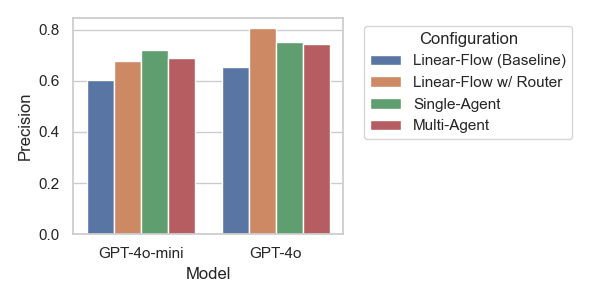
\includegraphics[scale=0.75]{images_exp2/precision/bar_best_precision_by_model_and_configuration.png}
                \caption{Best precision by model and configuration.}
                \label{fig:bar_best_precision_by_model_and_configuration}
            \end{figure}

            \subsubsection{Best Precision by Question Index and Configuration}
            \begin{figure}[H]
                \centering
                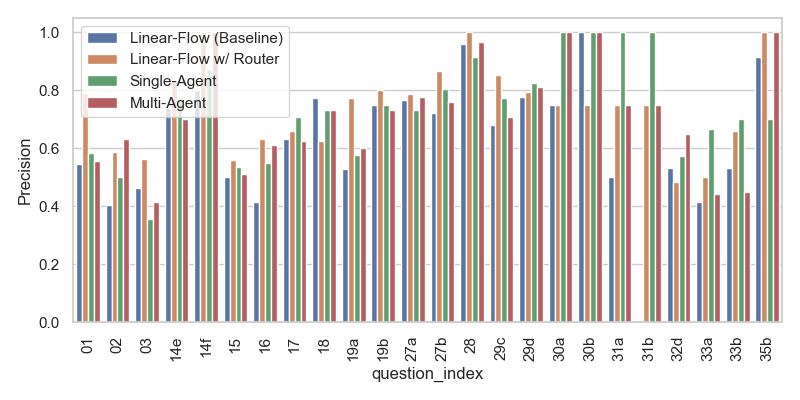
\includegraphics[scale=0.75]{images_exp2/precision/best_precision_by_question_index_and_configuration.png}
                \caption{Best precision by question index and configuration.}
                \label{fig:best_precision_by_question_index_and_configuration}
            \end{figure}

            \subsubsection{Best Precision by Question Index and Model}
            \begin{figure}[H]
                \centering
                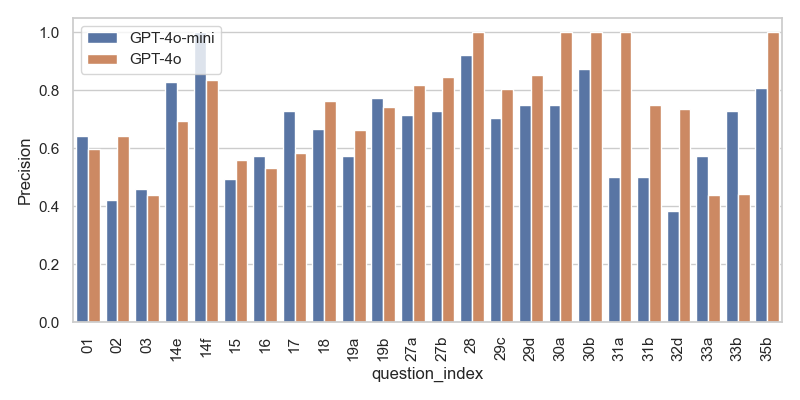
\includegraphics[scale=0.75]{images_exp2/precision/best_precision_by_question_index_and_model.png}
                \caption{Best precision by question index and model.}
                \label{fig:best_precision_by_question_index_and_model}
            \end{figure}

            \subsubsection{Facet Histogram of Precision by Model}
            \begin{figure}[H]
                \centering
                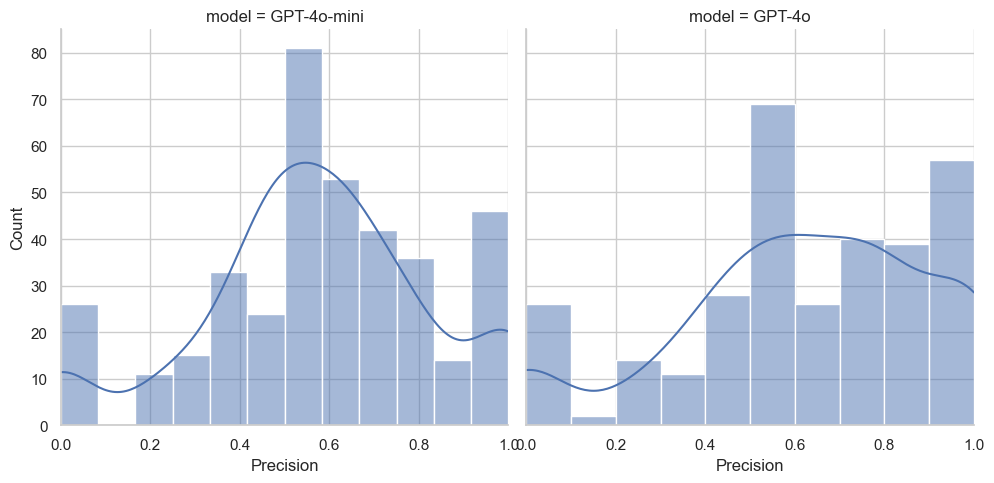
\includegraphics[width=\textwidth]{images_exp2/precision/facet_hist_precision_by_model.png}
                \caption{Facet histogram of precision by model.}
                \label{fig:facet_hist_precision_by_model}
            \end{figure}

            \subsubsection{Facet Histogram of Precision by Model (best of 3)}
            \begin{figure}[H]
                \centering
                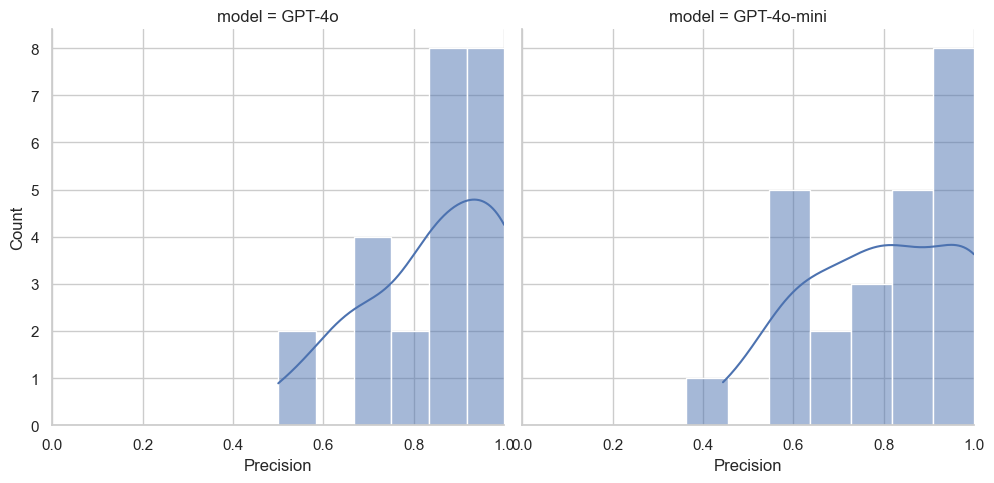
\includegraphics[width=\textwidth]{images_exp2/precision/facet_hist_precision_by_model_best_precision.png}
                \caption{Facet histogram of precision by model (best of 3).}
                \label{fig:facet_hist_precision_by_model_best_precision}
            \end{figure}

            % \subsubsection{Heatmap of Precision by Question and Model}
            % \begin{figure}[H]
            %     \centering
            %     \includegraphics[scale=0.75]{images_exp2/precision/heatmap_precision_by_question_and_model.png}
            %     \caption{Heatmap of precision by question and model.}
            %     \label{fig:heatmap_precision_by_question_and_model}
            % \end{figure}

            \subsubsection{Histogram of All Precisions}
            \begin{figure}[H]
                \centering
                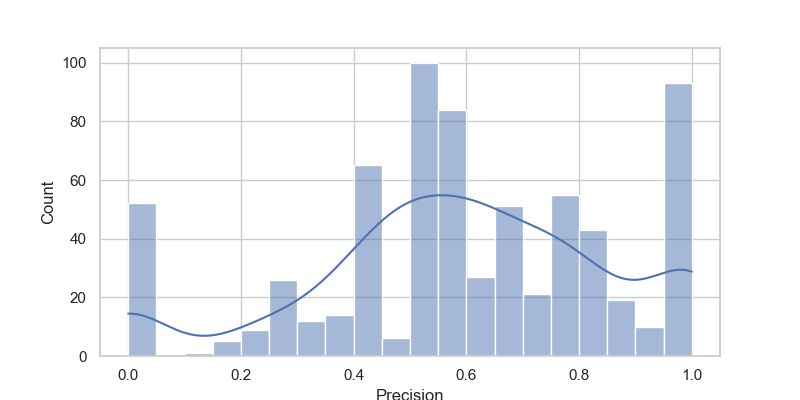
\includegraphics[scale=0.75]{images_exp2/precision/hist_precision_all.png}
                \caption{Histogram of all precisions.}
                \label{fig:hist_precision_all}
            \end{figure}

            \subsubsection{Line Plot of Precision by Question Index and Model}
            \begin{figure}[H]
                \centering
                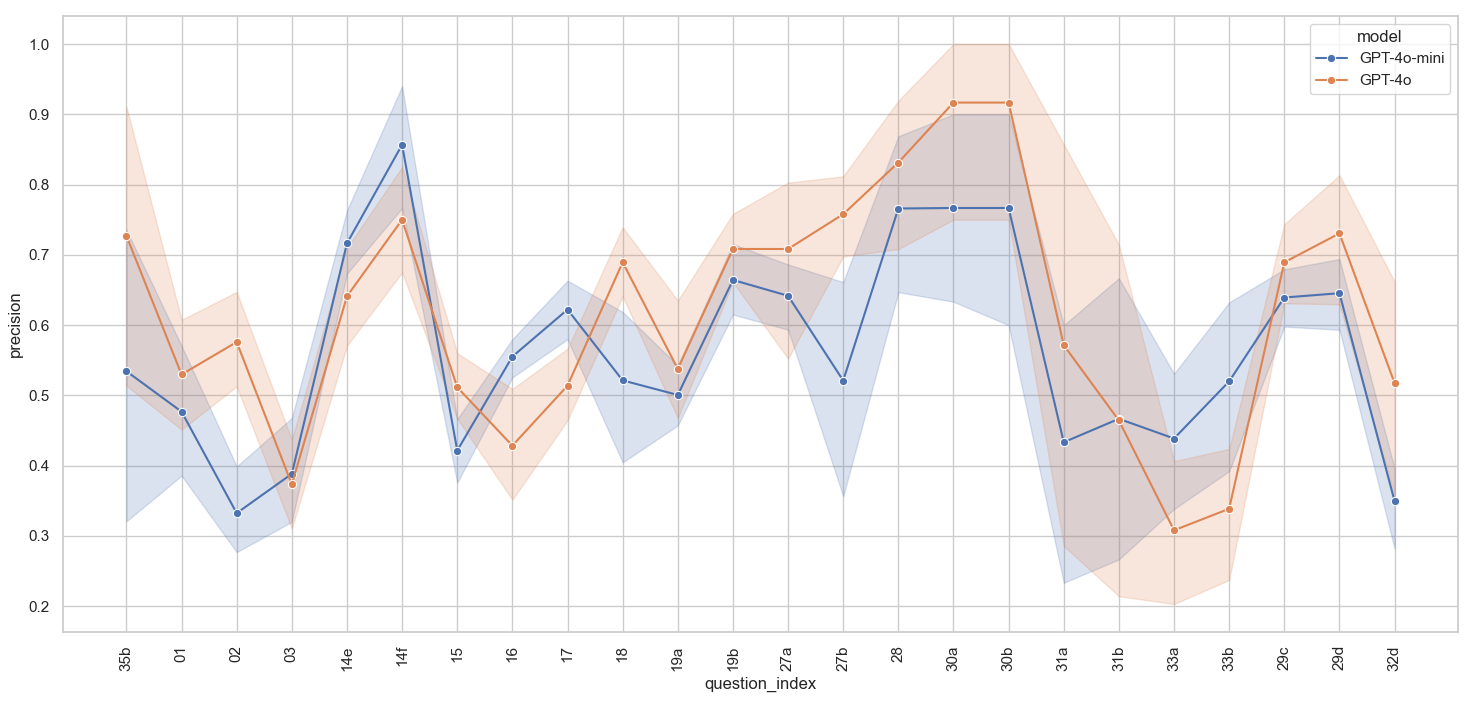
\includegraphics[width=\textwidth]{images_exp2/precision/line_precision_by_question_index_and_model.png}
                \caption{Line plot of precision by question index and model.}
                \label{fig:line_precision_by_question_index_and_model}
            \end{figure}

            \subsubsection{Boxplot of Precision by Model and Configuration}
            \begin{figure}[H]
                \centering
                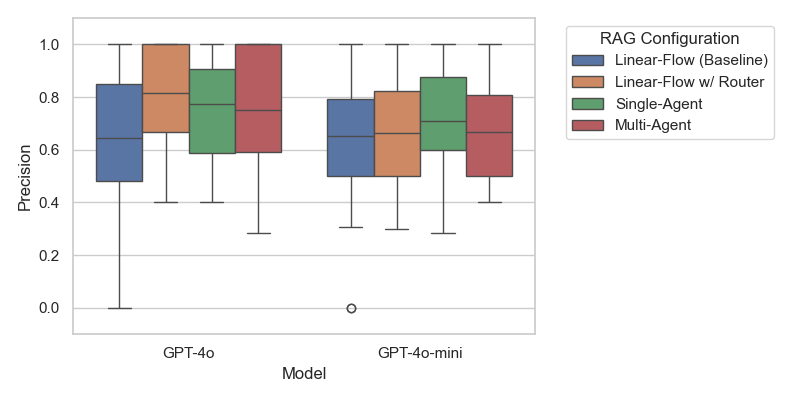
\includegraphics[scale=0.75]{images_exp2/precision/precision_boxplot_by_model_and_configuration.png}
                \caption{Boxplot of precision by model and configuration.}
                \label{fig:precision_boxplot_by_model_and_configuration}
            \end{figure}

            \subsubsection{Precision by Model}
            \begin{figure}[H]
                \centering
                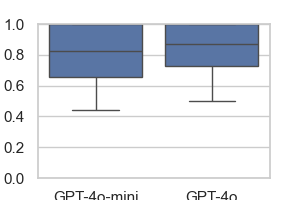
\includegraphics[scale=0.75]{images_exp2/precision/precision_by_model.png}
                \caption{Precision by model.}
                \label{fig:precision_by_model}
            \end{figure}

            \subsubsection{Precision by Model and Configuration}
            \begin{figure}[H]
                \centering
                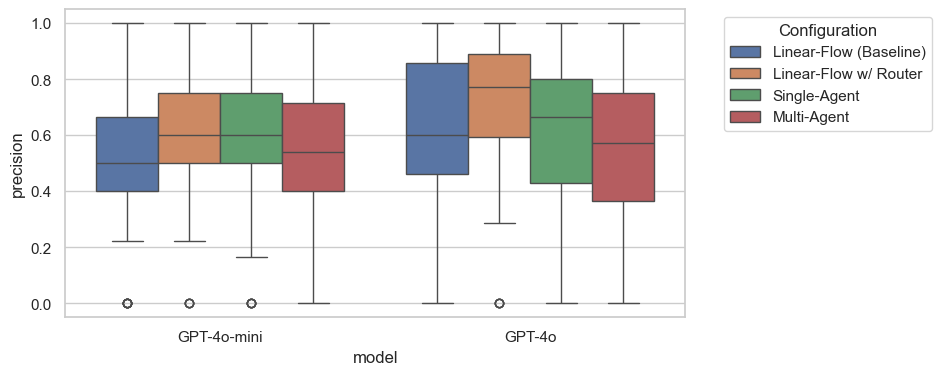
\includegraphics[scale=0.75]{images_exp2/precision/precision_by_model_and_configuration.png}
                \caption{Precision by model and configuration.}
                \label{fig:precision_by_model_and_configuration}
            \end{figure}

            \subsubsection{Line Plot of Precision by Question Index and Configuration}
            \begin{figure}[H]
                \centering
                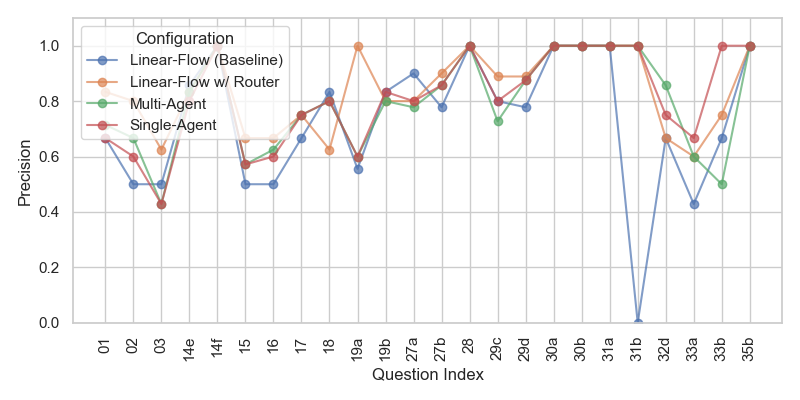
\includegraphics[width=\textwidth]{images_exp2/precision/precision_lineplot_by_question_index_and_configuration.png}
                \caption{Line plot of precision by question index and configuration.}
                \label{fig:precision_lineplot_by_question_index_and_configuration}
            \end{figure}

            \subsubsection{Scatter Plot of Precision vs. Total Time}
            \begin{figure}[H]
                \centering
                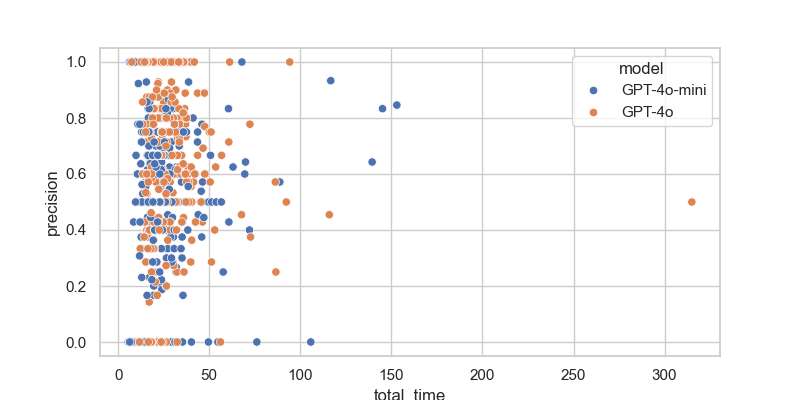
\includegraphics[scale=0.75]{images_exp2/precision/scatter_precision_vs_total_time.png}
                \caption{Scatter plot of precision vs. total time.}
                \label{fig:scatter_precision_vs_total_time}
            \end{figure}

            \subsubsection{Scatter Plot of Precision vs. Total Token Count Input}
            \begin{figure}[H]
                \centering
                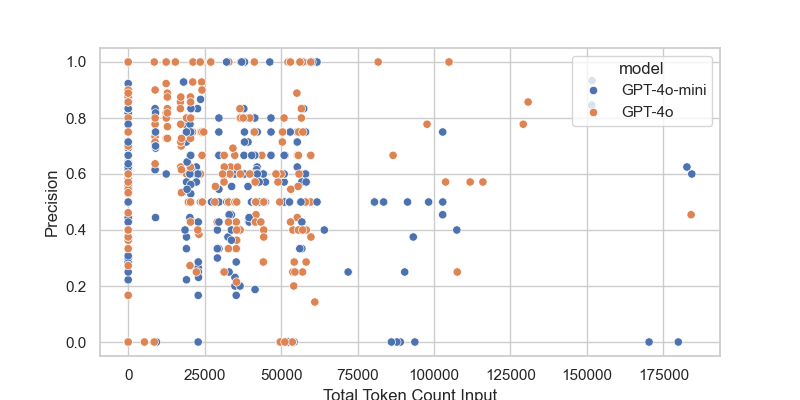
\includegraphics[scale=0.75]{images_exp2/precision/scatter_precision_vs_total_token_count_input.png}
                \caption{Scatter plot of precision vs. total token count input.}
                \label{fig:scatter_precision_vs_total_token_count_input}
            \end{figure}

            \subsubsection{Swarm Plot of Precision by Model and Configuration}
            \begin{figure}[H]
                \centering
                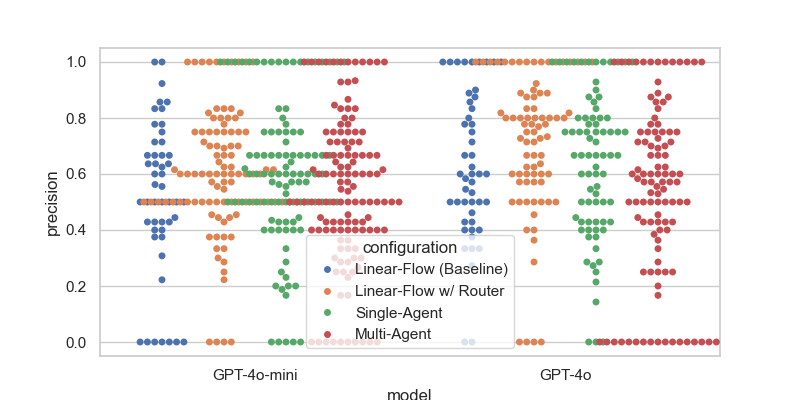
\includegraphics[scale=0.75]{images_exp2/precision/swarm_precision_by_model_and_configuration.png}
                \caption{Swarm plot of precision by model and configuration.}
                \label{fig:swarm_precision_by_model_and_configuration}
            \end{figure}

            \subsubsection{Violin Plot of Precision by Model and Configuration}
            \begin{figure}[H]
                \centering
                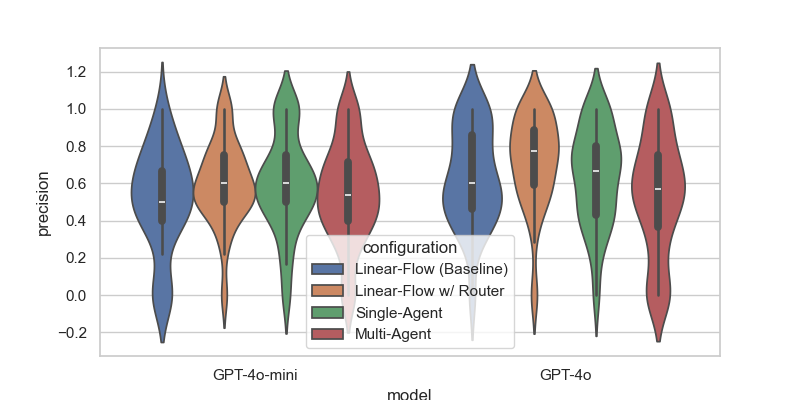
\includegraphics[scale=0.75]{images_exp2/precision/violin_precision_by_model_and_configuration.png}
                \caption{Violin plot of precision by model and configuration.}
                \label{fig:violin_precision_by_model_and_configuration}
            \end{figure}

        % \subsection{Recall}

        %     TEXT

        %     ...

        %     ... 

            
        %     TEXT

        %     ...

        %     ... 

        